\DeclareUnicodeCharacter{2028}{} 
\documentclass{article}
\usepackage[dvipsnames]{xcolor}
\usepackage{listings}
\usepackage[section]{placeins}
\usepackage{blindtext}
\usepackage[T1]{fontenc}
\usepackage[utf8]{inputenc}
\usepackage{titling}
\usepackage{float}
\usepackage{tikz}
\usetikzlibrary{calc}
\usetikzlibrary{arrows.meta}
\usepackage{graphicx}
\usepackage[hidelinks]{hyperref}





\title{ Design Document\\2020-2021}
\author{Alessandro Polidori (Codice persona 10573078)\\Olimpia Rivera (Codice persona 10617517)}
\date{}



\renewcommand{\contentsname}{Table of Contents}


\begin{document}

\renewcommand{\labelitemi}{\normalfont -} 

\begin{figure}[]
  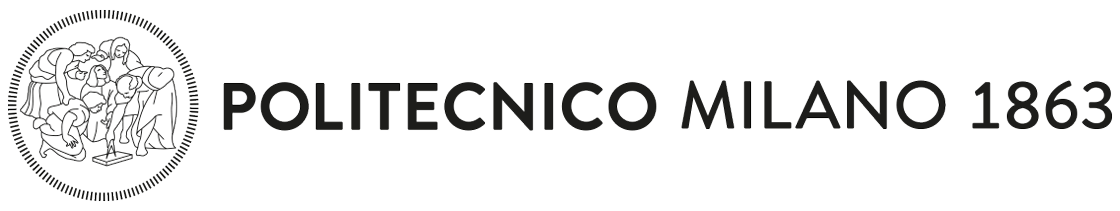
\includegraphics[width=\linewidth]{logo_politecnico copia.png}
  
\end{figure}
\maketitle
\tableofcontents{}
\newpage

\section{Introduction}
\subsection{Purpose}
The purpose of this document is to further detail the software system discussed in the RASD by providing more technical and precise informations. The RASD, indeed, describes the system in terms of requirements, assumptions and goals and gives a general overview of the main system’s functionalities, whereas the DD goes deeper into software design and architecture. In particular, all the required components of the system and the interactions among them are presented, as well as run-time processes and motivated design choices. In addition, the document describes the implementation, integration and testing plans.\\
The relevant issues explored in the Design Document are the following:
\begin{itemize}
\item High-level architecture
\item Main components and relative interfaces
\item Runtime behavior
\item Design patterns
\item Implementation, integration and testing plan
\end{itemize}
This document represents a vehicle for stakeholders communication, as it defines a set of design  decisions made to offer both the essential functionalities and the required quality attributes.

\subsection{Scope}
The CLup software application is designed to help both common users and store managers to deal with some relevant difficulties and challenges created by the coronavirus emergency. The CLup system, indeed, gives users the possibility to join virtual lines to stores and wait for their turn at home instead of standing in line outside stores. The system itself notifies users when it is time to leave to reach the store. Alternatively, thanks to the CLup application, users can choose to book visits to stores in advance, by selecting the preferred date and time slot.
 In order for the lining up mechanism to work effectively, all the users are asked to provide their expected shopping duration and the system will calculate, and eventually modify, the waiting times of the users in line by taking into account the following events: users currently in line, users currently in the store, users getting out of the line, cancelled reservations, crowdedness of stores’ departments and users’ visits’ durations. Indeed, a QR code will be generated for each user and scanned at entrances and exits by smart turnstiles, so that the system can collect and store informations about visits’ duration. The influx of people is managed by the system in an even finer way, by asking users to provide a list of product categories they intend to purchase. The system is also designed to regulate accesses to stores in order to respect restrictions imposed by the virus emergency, by taking into account the stores’ capacities. For this reason, store managers as well benefit from such a software application because they have the possibility to monitor the number of people in they stores updating in real time.\\
A more detailed overview of the functionalities offered by the system can be found in the RASD.

\subsection{Definitions, Acronyms, Abbreviations}
\subsubsection{Definitions}
\subsubsection{Acronyms}
\begin{itemize}
\item RASD: Requirements Analysis and Specifications Document
\item DD: Design Document
\item API: Application Programming Interface
\item DBMS: Database Management System
\item RDBMS: Relational Database Management System
\item RMI: Remote Method Invocation
\item JDBC: Java DataBase Connectivity
\end{itemize}
\subsubsection{Abbreviations}
\begin{itemize}
\item Rn: n-th functional requirement
\end{itemize}
\subsection{Revision History}
\subsection{Document Structure}
The Design Document is structured in the following chapters:
\begin{itemize}
\item\textbf{Chapter 1} describes the document’s purpose and scope and its differences with respect to the RASD. Useful specifications (definitions, acronyms, abbreviations) are included for a better understanding of the next sections of the document.
\item\textbf{Chapter 2} represents the core section of the document because it deals with the architectural design choices. In particular, it describes all the system's components, their interfaces, how they are distributed on physical nodes and the interactions among them. It also presents the methods provided by the component's interfaces and how they are used in different processes. Finally, chapter 2 provides a description of the selected architectural styles and patterns, together with the reasons why they have been chosen.
\item\textbf{Chapter 3} it provides some relevant UX diagrams to further detail the interaction between users and the application presented in the RASD.
\item\textbf{Chapter 4} identifies by which component each of the system's requirement (defined in the RASD) is satisfied.
\item\textbf{Chapter 5} describes the plans that have been chosen for the following crucial activities: implementation, integration and testing.
\item\textbf{Chapter 6} presents the effort spent by the group members while working on this project.
\item\textbf{Chapter 7} includes the reference documents.
\end{itemize}

\section{Architectural Design}
\subsection{Overview}
The application architecture is going to be developed as a three-tier architecture. The three logical and physical computing tiers are the following:
\begin{itemize}
\item\textbf{Presentation Tier:} manages the interaction between users and the application. It is responsible for collecting informations from the users and for displaying informations.
\item\textbf{Business logic or Application Tier:} it is where all the communication goes through: it is in charge of processing information collected in the presentation tier and passing it to the data tier. It also manages the way functions are presented to the users.
\item\textbf{Data Access Tier:} it stores and manages the informations processed by the application by performing the necessary operations into the database.
\end{itemize}
More precisely, the architecture is made as a three-tier client-server style, in which presentation, application logic and data processing layers are divided across client and server devices and they all have their own dedicated hardware. The advantages for choosing such an architecture will be further explained in the next sections.
\smallskip\\
Depending on the functionality requested by a user, the client requests a certain service from the server and the invocation of different methods takes place. The server itself provides the needed services through well defined APIs.
\smallskip\\
The functionalities offered by CLup work in the following way:
\begin{itemize}
\item\textbf{Line up:} the application server receives a request of lining up, it takes the required information about the current state of the line from the database server and it sends it back to the client. If the user decides to line up, the application server will communicate with the database server to store the information about the new user, so that the state of the line can be changed. 
\item\textbf{Book visit:} the application server receives a request for booking a visit and provides the user with the necessary forms to complete the reservation. The informations provided by the users will be sent to the application server and then stored in the database.
\item\textbf{Check counter:} the application server will receive the request from the store manager’s client, it takes the information about the counter from the database server and it sends it back to the client.
\item\textbf{Print ticket:} whenever a store manager decides to print a physical ticket, the application server will inform the database server in order for the state of the line to be correctly updated.
\end{itemize}
\subsection{High Level Components}
The following figure represents an high level architecture of the system, showing the different physical machines dedicated to each of the three logic software layers: a tier to interface with the user, a middle tier that holds the business logic of the system, which separates clients and data, and a DataBase Server for the data access layer that holds all the data of the application. \\
\smallskip\\
Not only the modularization of the three layers provides many benefits in terms of flexibility for developers, by allowing them to work on specific part of the application, with minimal impact on the other layers, but it also guarantees more secure accesses to the database. To enhance the overall security of the system, firewalls are installed to monitor and control incoming and outgoing network traffic.
\smallskip\\
Another great advantage of this type of architecture that is exploited is scalability: Application Server and Web Server nodes are replicated and a load-balancing systems are added, improving the overall performance. Note that the Application server and the Web server are considered as a single middle tier containing the business logic, according with the previously defined three-tier architecture. It must be remarked, however, that the Web Server is only used to provide static content (HTML pages).
\smallskip\\
Additionally, reliability and availability are also increased by the usage of a cache on the client side. Indeed, to fasten the process of store selection, the users’ mobile app stores the list of all shops, in order to avoid the connection to the Internet to retrieve the desired one. Consequentially, a mechanism able to keep data up to date is needed.
\smallskip\\
Finally, the clients configuration considered is the Thick one, because it also contains a small part of the business logic. In particular, the clients are able to compute the function that checks whether the waiting time equals the time needed by the user to reach the store. For this reason, the (asynchronous) notification received by the user when it is time to reach the store, is completely managed on the client side.
\smallskip\\
The figure below provides a more detailed, but still very high-level architectural overview, also showing the interaction among the various components.\\
\smallskip\\
\begin{figure}[H]
  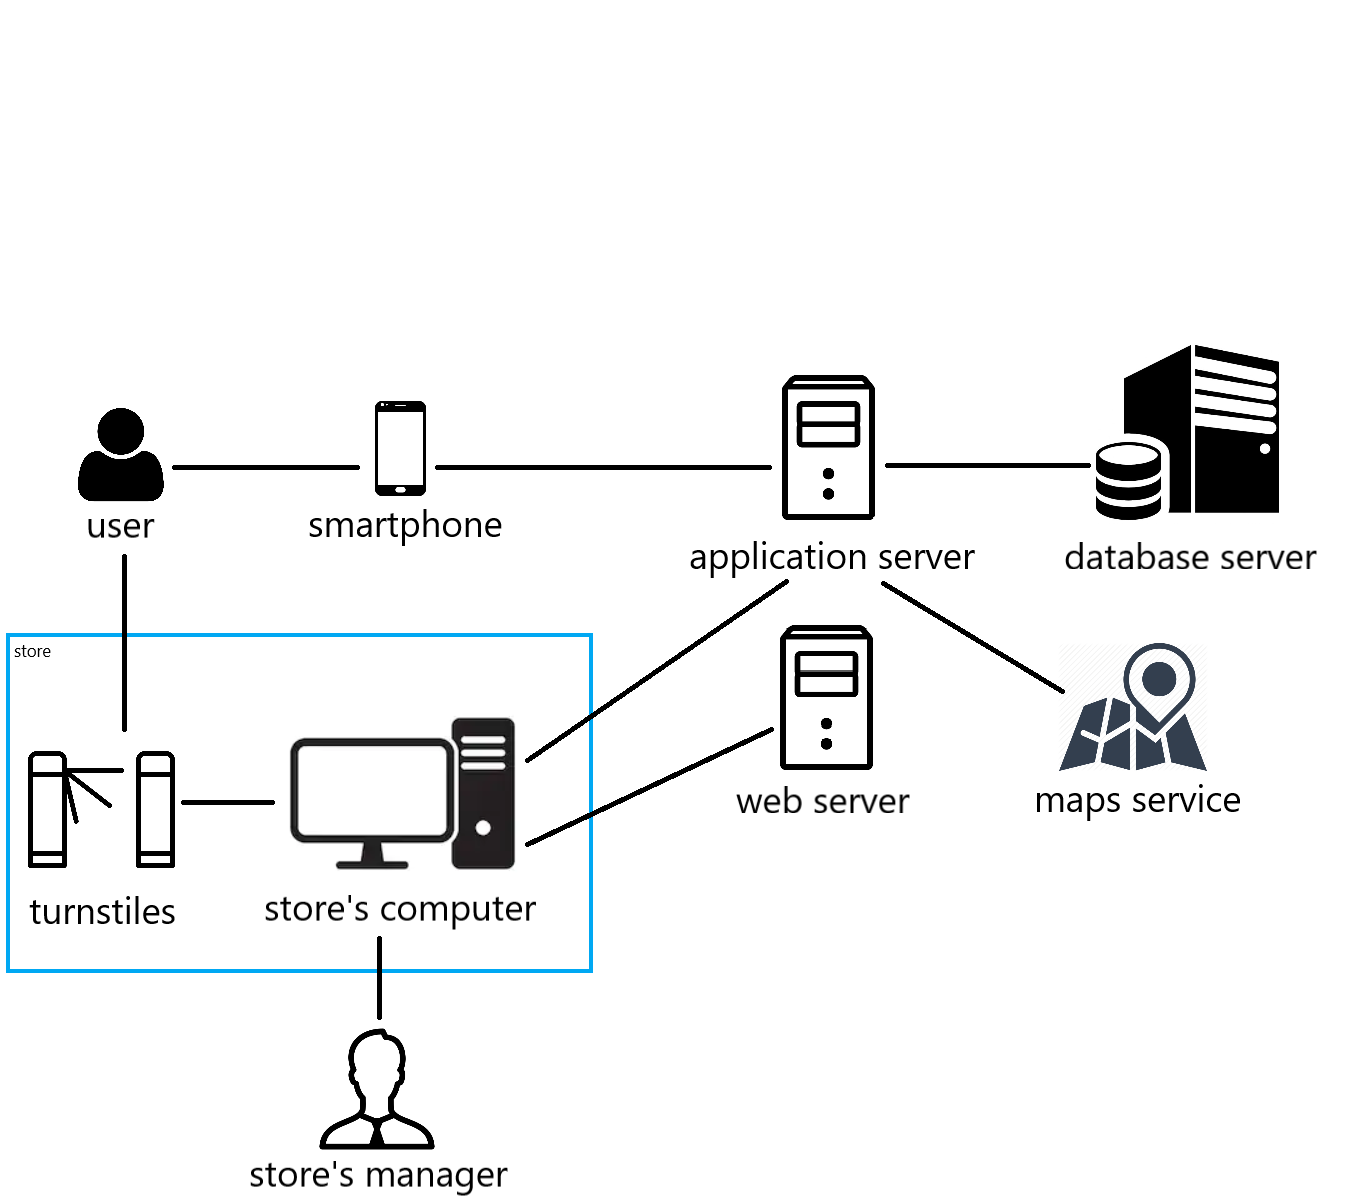
\includegraphics[width=\linewidth]{highArchitecture.png}
  
\end{figure}
As shown in the image, clients’ devices can be either smartphones (for store’s customers), which are connected to the Application Server, or computers (for store’s manager). The Web Servers are used to manage communication with store’s managers’ Web applications: it forwards requests to the Application Server, which ultimately communicates with the Database Server. The Application Server also exploits a Maps service API in order to retrieve users’ locations.
\subsection{Component view}
In the diagram below, the main software components and their relations are shown. Only application server's
components and offered interfaces are analyzed in detail. It is important to point out that this is only a
suggested components' structure, useful to understand how the components communicate with each other,
and that it could be implemented in many different ways.
\begin{figure}[H]
  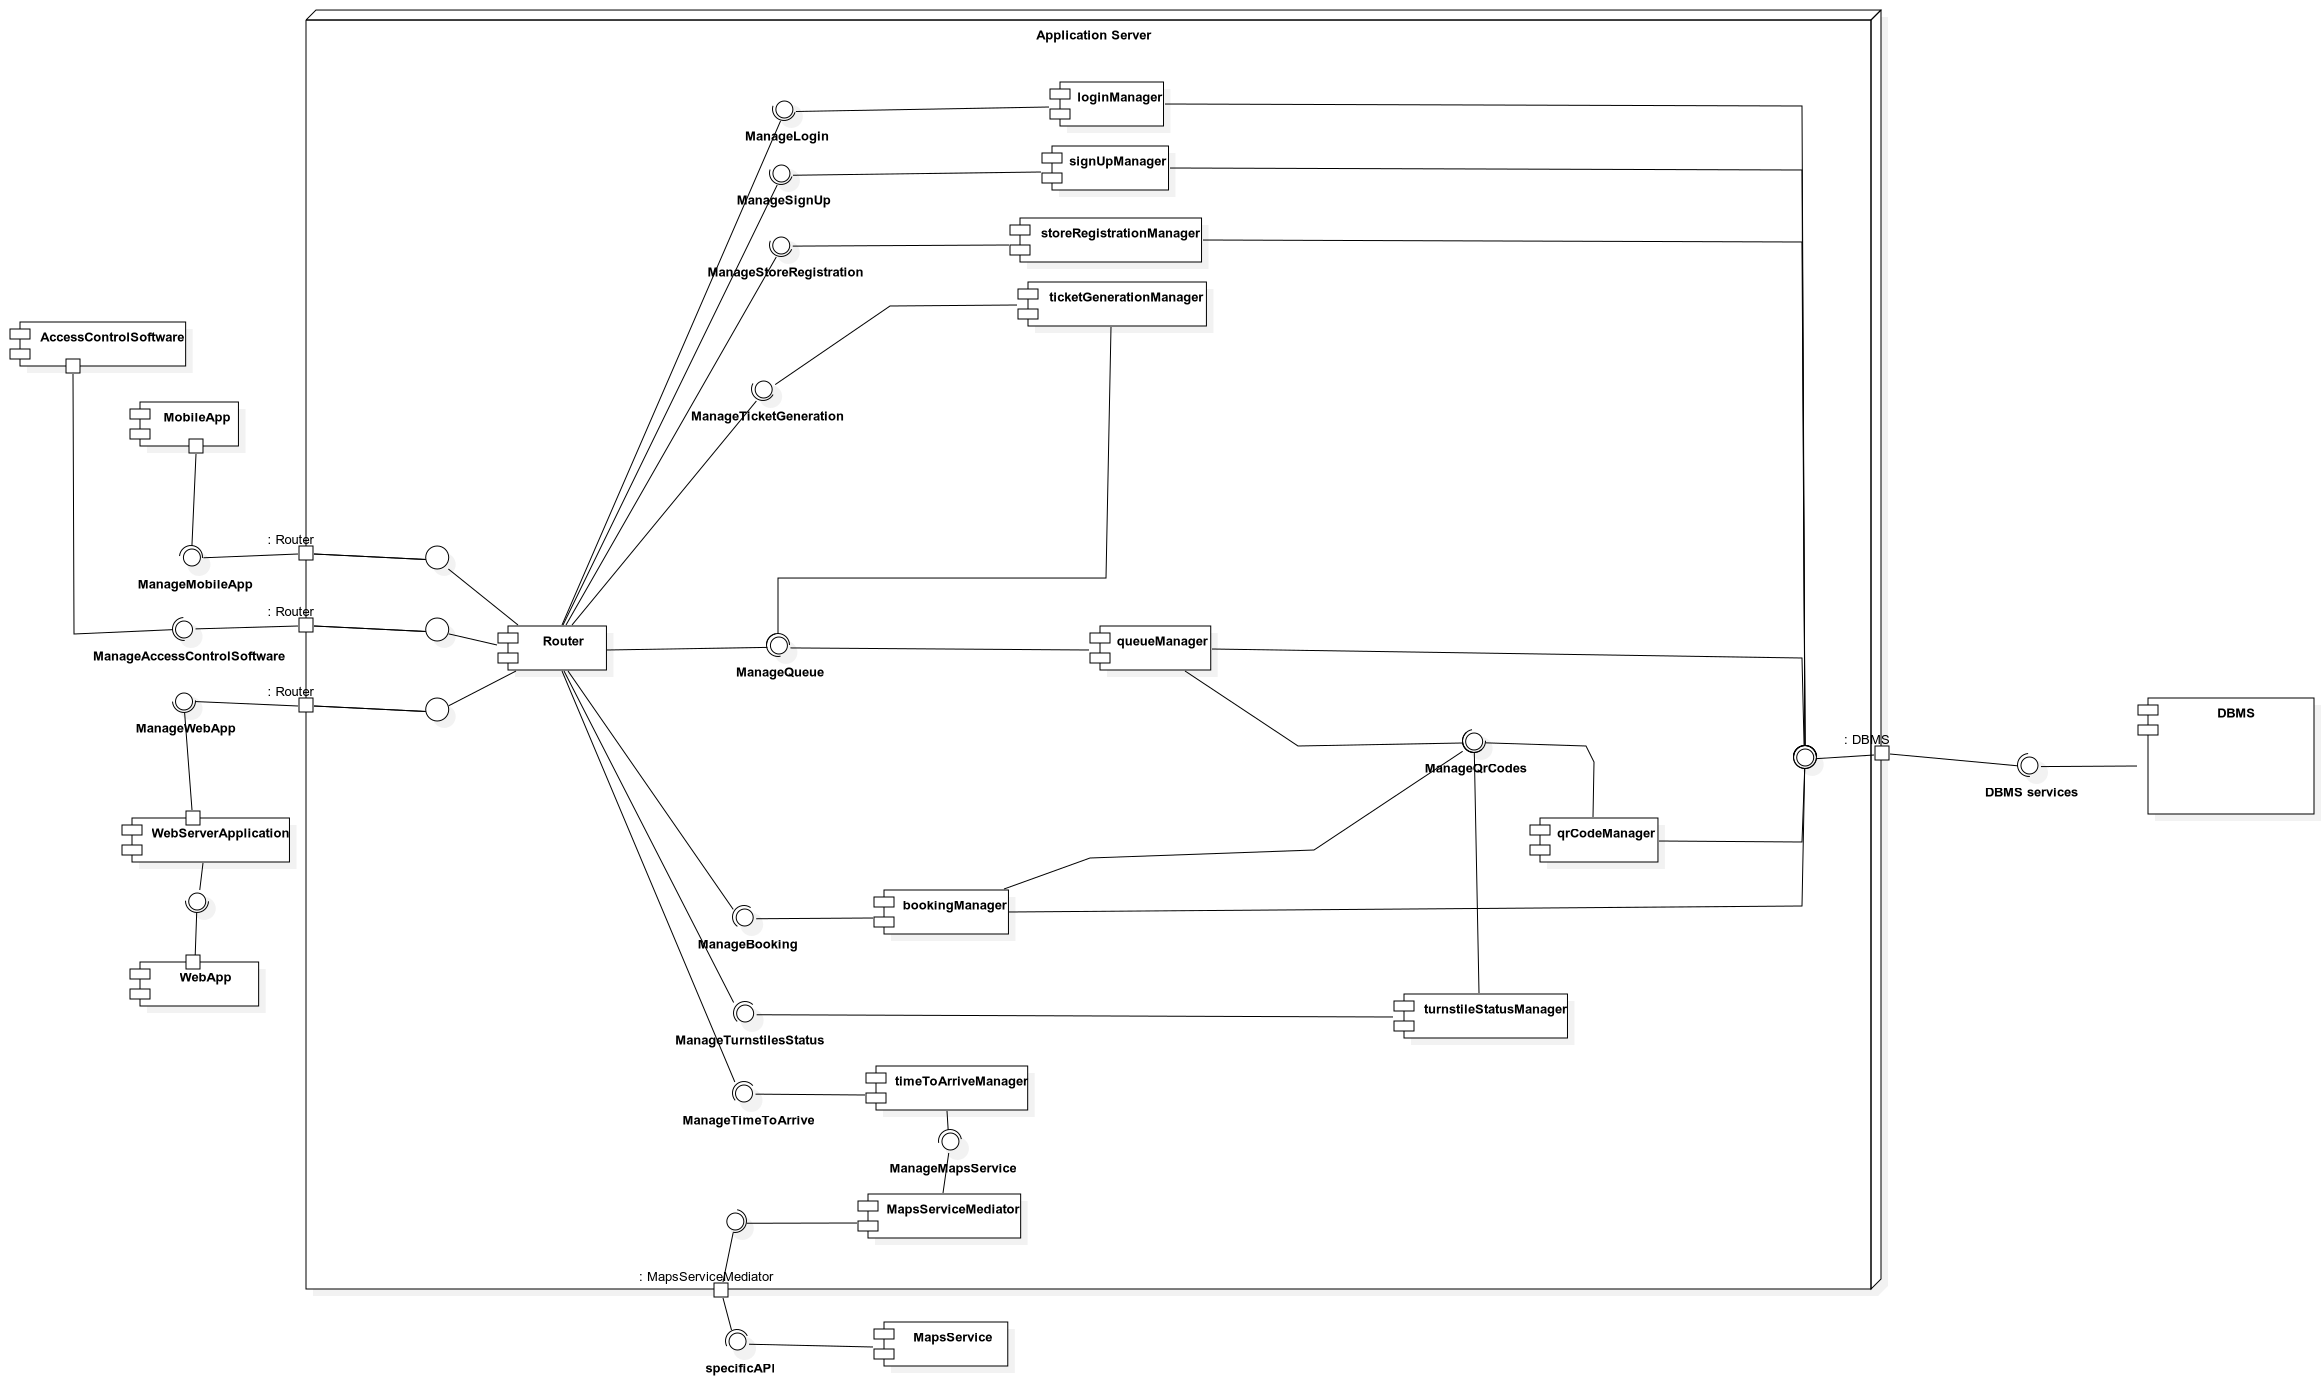
\includegraphics[width=\linewidth]{ComponentDiagram.png}
  
\end{figure}

\begin{itemize}
\item\textbf{loginManager}: this component manages the logic behind the mobile user's and storemanager's authentication.
It needs to access the database in order to check if the credentials are valid.
\item\textbf{signUpManager}: it manages the mobile user's initial sign-up. It access the database to retrieve the sign-up
form and to save the new user's credentials.
\item\textbf{storeRegistrationManager}: it controls the storemanager's initial registration of himself and, therefore,
of the store. It has to interact with the database in a similar way to the signUpManager component, but it 
needs also to manage the logic behind the validation of the storemanager's identity.
\item\textbf{ticketGenerationManager}: this component creates tickets. It needs to add one more person to the virtual
queue, so it communicate with the queueManager component in the same way "mobileApp" does when
a user decides to get in line using his smartphone app.
\item\textbf{queueManager}: this component controls all the operations involving the virtual line. It also includes
the waiting-times managing algorithm. It access the DBMS to retrieve queues' data, information regarding the current state of the line, data regarding shopping duration/ product lists and to store the current state of the line. It is also the responsible of the calculation of the inferred shopping duration.
\item\textbf{qrCodeManager}: it manages the creation of new QRCodes, the validity check and it stores data regarding
the mapping between codes and reservations/turnNumbers.
\item\textbf{bookingManager}: it manages all the logic behind booking process. It stores new reservations.
\item\textbf{turnstileStatusManager}: it manages the turnstile status. It unlocks them if the scanned QrCode is valid, so
it has to interact with qrCodeManager.
\item\textbf{timeToArriveManager}: its purpose is to manage the information regarding the geolocation and correlated details like distance and time to arrive. In this first version of CLup it does nothing more than forward time-to-arrive request to the mapsServiceMediator.
\item\textbf{MapsServiceMediator}: the purpose of this component is to decouple the system from a specific maps service, so future external changes won't affect the internal system's interface.

\end{itemize}
\subsection{Deployment View}
In the following deployment diagram the actual physical nodes of the system and the type of used hardware are represented. It also shows the communication methods that occur among the components.\\

\begin{figure}[H]
  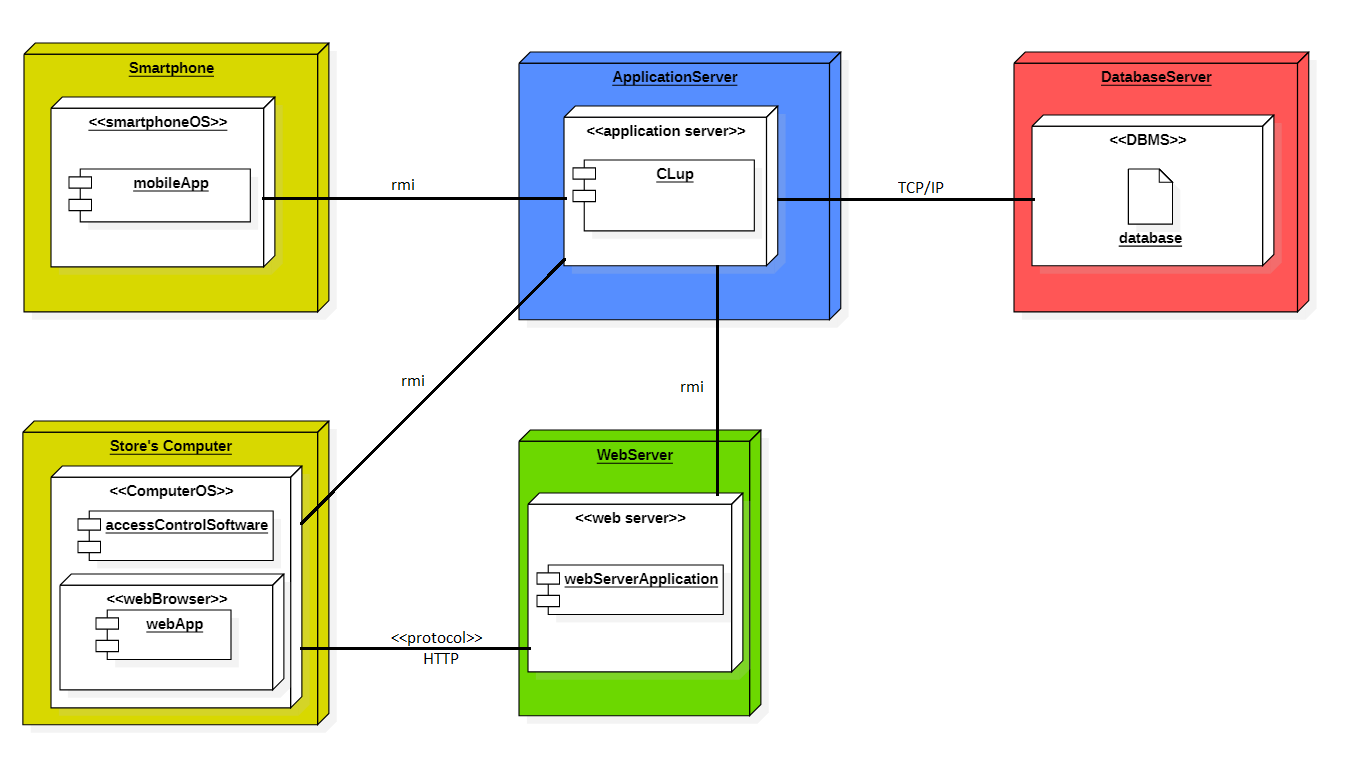
\includegraphics[width=\linewidth]{deployment.png}
  
\end{figure}

The nodes show in the image above are the following:
\begin{itemize}
\item\textbf{Smartphone:} together with the store’s computer, it is part of the first tier in which presentation logic must be deployed. The user accesses CLup’s services though this type of device, that communicates with the Application Server, using RMI technology. The mobile application must be compatible with the most of the existing Operating Systems, in order to be available on most of the devices.
\item\textbf{Store’s computer:} it is used by store managers (or their employees) to ask for and receive data on the actual crowdedness of their stores and to send informations regarding the printing of physical tickets. The communication between the Web Application and the Web Server takes place through the HTTP protocol. The Web Application must be compatible with the most popular Web Browsers.
Additionally, on this same node, a piece of software that communicates with the turnstiles' firmware is deployed. This Access Control Software communicates with the Application Server through RMI, in order to keep the customer counter updated. The Application Server, indeed, receives informations about entrances from it, which will eventually be forwarded to the database, in order to keep the state of the store’s crowdedness updated. This piece of software must be able to communicate with the most common turnstiles’ brands.
\item\textbf{Application Server:} it is where most of the application logic is deployed. The mobile application directly forwards all the requests to it, in order to receive the appropriate services. It also handles requests coming from the Web Server, sent by the Web Application. The Application Server is what enables the communication between the Database Server and both the mobile phone and the store's computer. Application Server and Database Server communicates through the JDBC protocol.
\item\textbf{Web Server:} it is always part of the middle tier, together with the Application Server. As stated before, however, requests that involve dynamic content (generation of tickets and customer counter), cannot be served by the Web Server. For this reason, these type of requests are forwarded to the Application Server.
\item\textbf{Database Server:} it stores and manages personal users’ data as well as the data relative to reservations and visits’ durations. It hosts a relational DBMS (RDBMS): it is the most suitable option for insertion, update and deletion of small amounts of data. It easily supports large number of users and frequent queries.
\end{itemize}
\subsection{Runtime View}
The following sequence diagrams represent the dynamic interactions among the components during relevant processes.
Note that, from this point on, Google Maps has been chosen as mapping and location provider among the other available ones. If offers a large library of APIs, which can be easily exploited for future additional functionalities. As stated in the RASD indeed, users are supposed not to change location while waiting for their turns, but things might change when the pandemic emergency will be over. For this reason, Google Maps would offer good quality services when dealing with real time changing locations. In addition, the Map Service can be easily replaced, without affecting the application internally, thanks to the presence of the MapsServiceMediator.
\begin{figure}[H]
  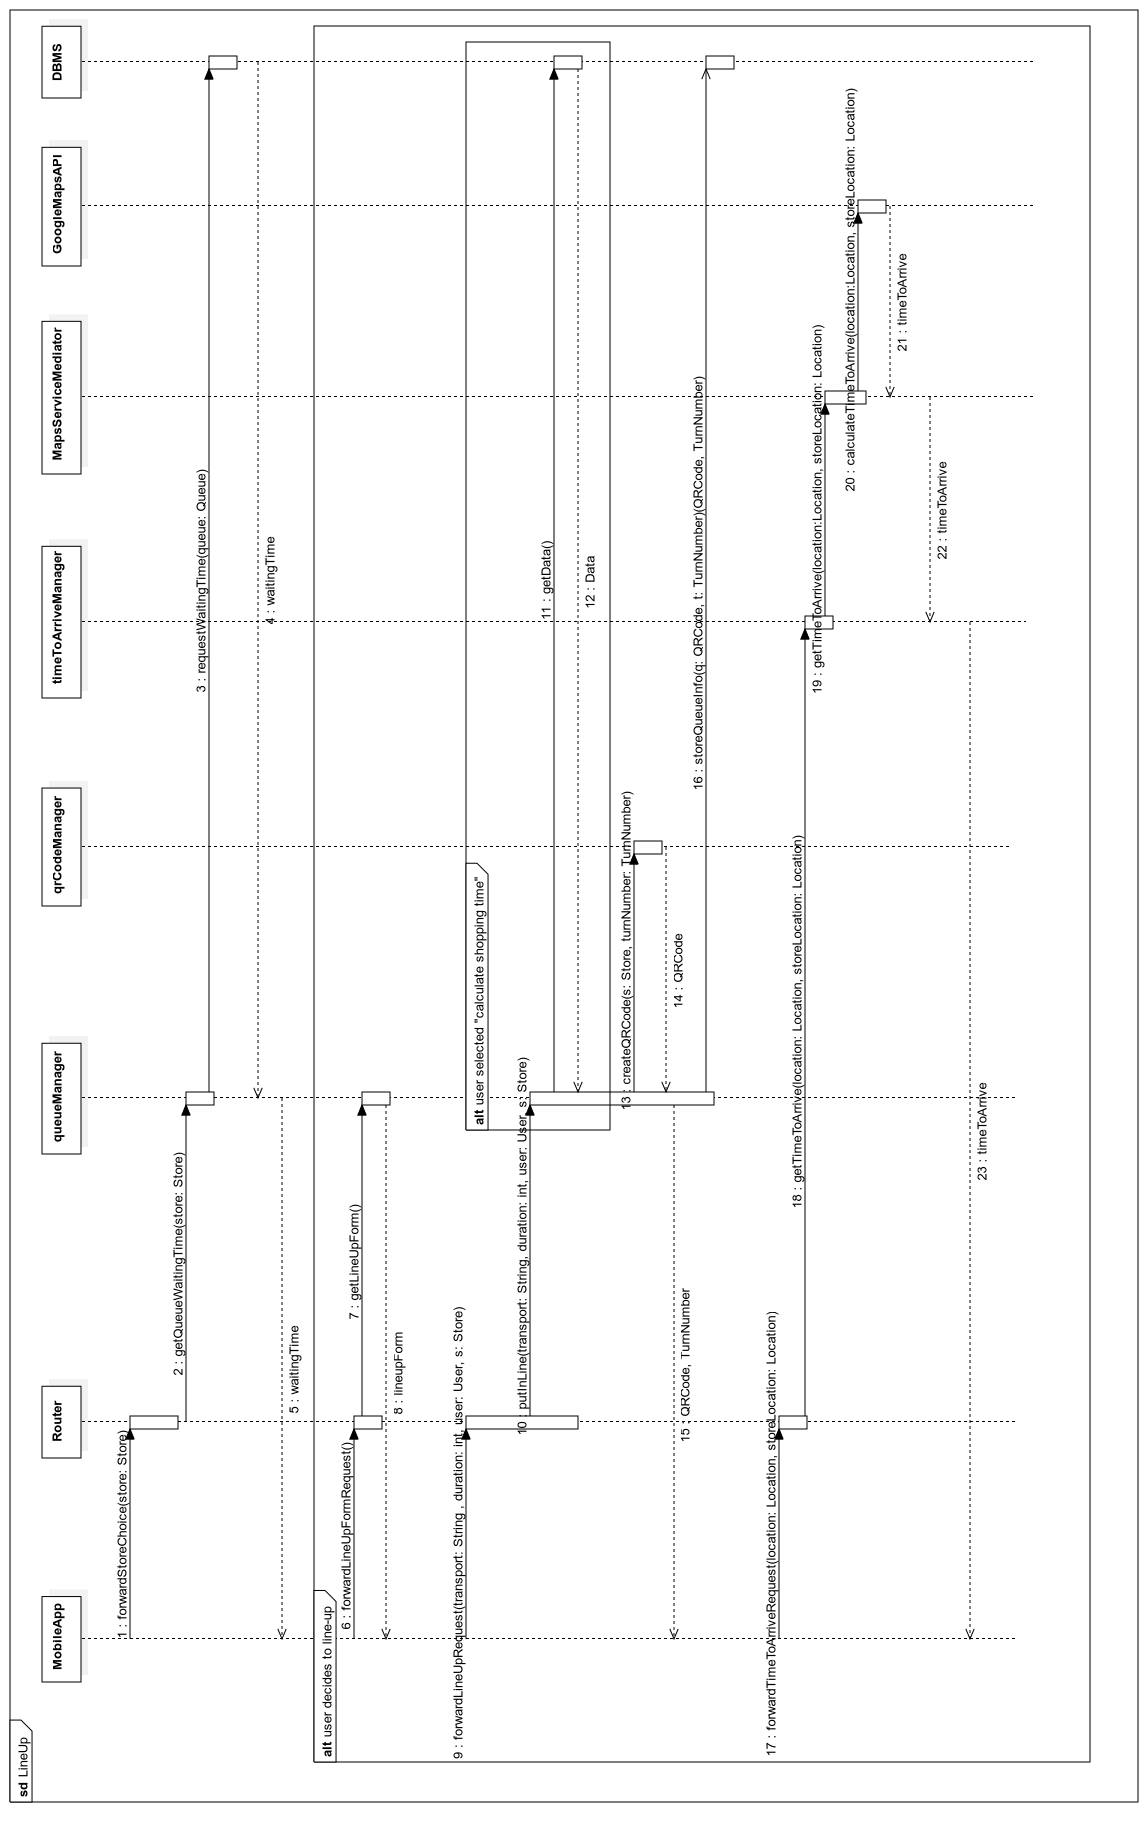
\includegraphics[width=\linewidth]{LineUpRT.png}
  
\end{figure}

\noindent This sequence diagram describes the process of getting into a store’s line. The user is assumed to be already logged in and to have already chosen the store. The user’s request to join a line is forwarded by the MobileApp to the Router, which, in its turn, forwards it to the QueueManager component. The QueueManager contacts the DBMS to receive the waiting time for that specific store, which is then forwarded to the MobileApp and shown to the user. At this point, if the user decides to line up, he/she inserts the rest of the mandatory informations (expected visit’s duration and means of transport), which are forwarded to the QueueManager. If the user has chosen to let the system infer his/her shopping time (based on his/her previous visits), the BookingManager contacts the DBMS in order to receive such an information, which is sent back to the Router. The Router itself, forwards to the QueueManager the request to finally put the user in line. The QRCodeManager is asked by the QueueManager to generate a QR code, uniquely associated to a certain turn number. The QueueManager is also in charge of notify the DBMS to store the new line’s informations. The QR code, together with the turn number are then rendered to the user through the MobileApp. The MobileApp sends to the router the request to calculate the time needed by the user to reach the store form his/her current location. This request is sequentially forwarded to the TimeToArriveManager and to the MapServiceMediator, which uses GoogleMapsAPI to retrieve this information, which is sent back to the MobileApp and shown to the user.
\begin{figure}[H]
  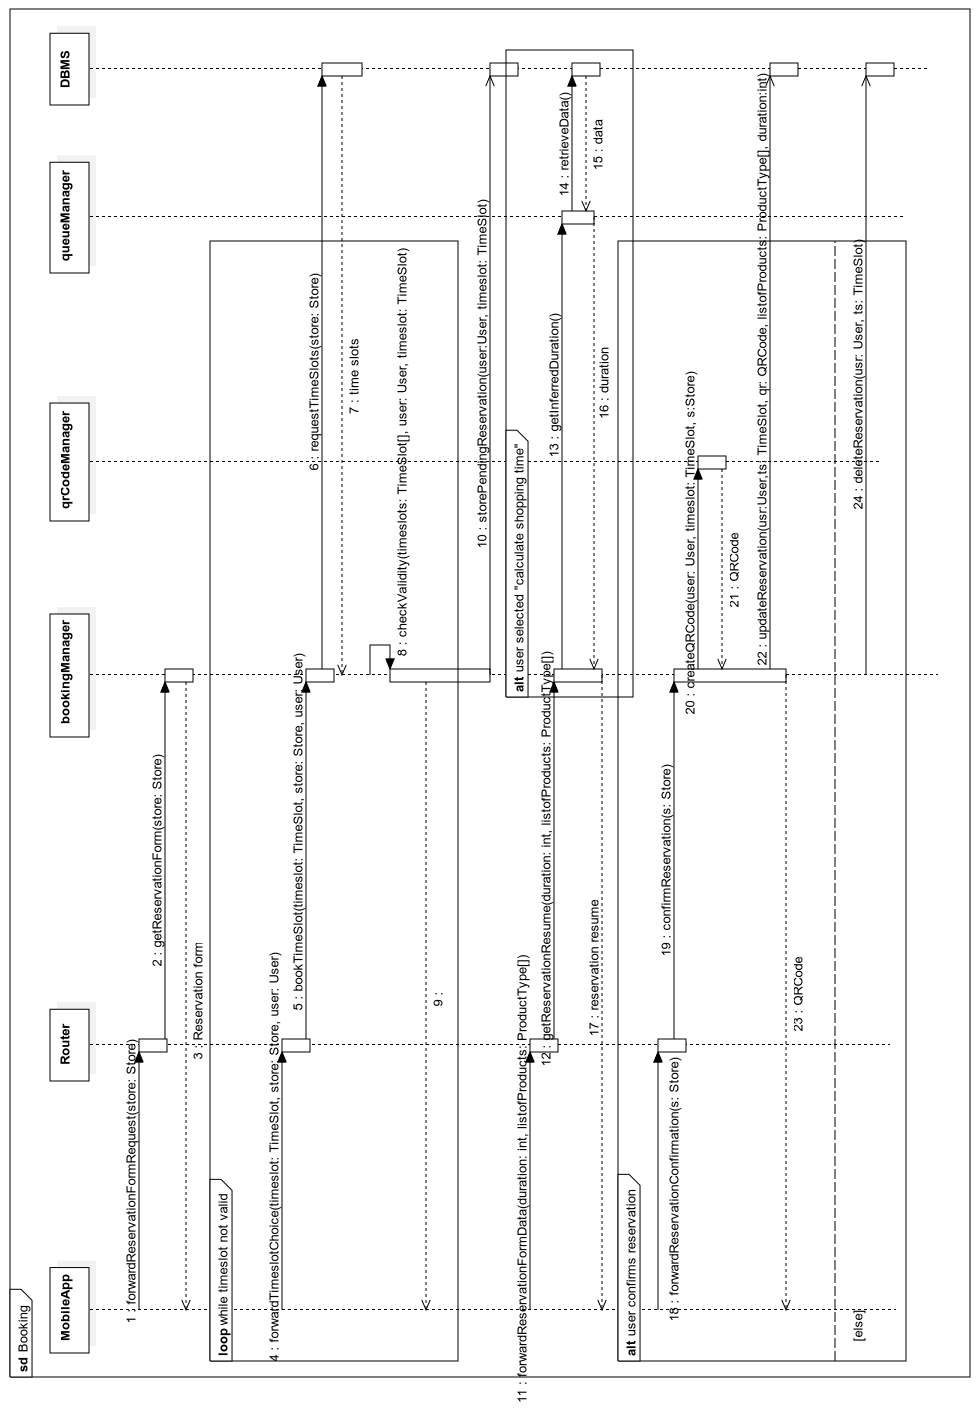
\includegraphics[width=\linewidth]{BookingRT.png}
  
\end{figure}
\newpage

\noindent The sequence diagram above shows the process of booking a visit. The user is assumed to be already logged in and to have already chosen the store. The user’s request to book a visit is forwarded by the MobileApp to the Router, which, in its turn, forwards it to the BookingManager component. A registration form is created and sent back to she user. As soon as the user inserts the preferred time slot, the BookingManager communicates with DBMS in order to check whether the time slot is valid (not overlapping with other use’s reservations. As soon as a valid time slot is selected by the user, a pending reservation is saved in the database and the MobileApp allows the users to fill the rest of the mandatory fields (expected visit’s duration and list of product types), which are forwarded to the BookingManager. As for the lining up process, if the user has chosen to let the system infer his/her shopping time (based on his/her previous visits), the BookingManager contacts the DBMS in order to receive such an information, which is added to the reservation resume sent to the user. Finally, if the user clicks on “confirm”, the BookingManager “tells” the DBMS to update and store the final reservation and sends to the QRCodeManager a request for generating a QR code for that specific user and time slot. The MobileApp renders the generated QR code to the user. In case the user does not confirm the reservation, the BookingManager warns the DBMS to delete the previous pending reservation.
\begin{figure}[H]
  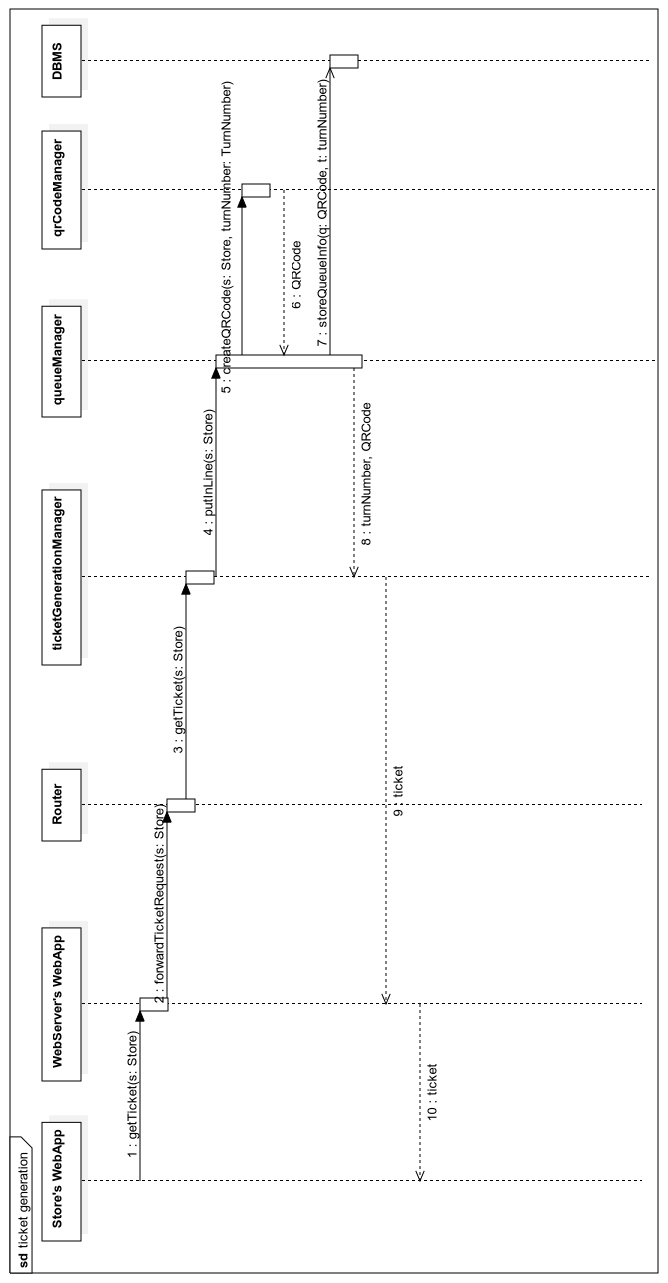
\includegraphics[width=\linewidth]{ticketRT.png}
  
\end{figure}

\noindent This sequence diagram describes what are the components needed when a physical ticket is printed and the interaction among them. The system has to take into account the people that reach the stores without the required technology, in order to keep the lines properly updated. A store manager makes a request through the Store’s WebApp to generate a ticket preview. The WebServer’s WebApp sends such a request to the Router, which forwards it to the TicketGenerationManager. At this point, the TicketGenerationManager communicates with the QueueManager, which is in charge of: asking the generation of a new QR code to the QRCodeManager and notifying the DBMS to store the new line’s  informations. The QR code, together with the turn number are sent back to the TicketGenerationManager, which finally generates and sends to the WebServer’s WebApp the ticket preview. The Store’s WebApp as well receives the ticket preview and renders it to the store’s manager.
\begin{figure}[H]
  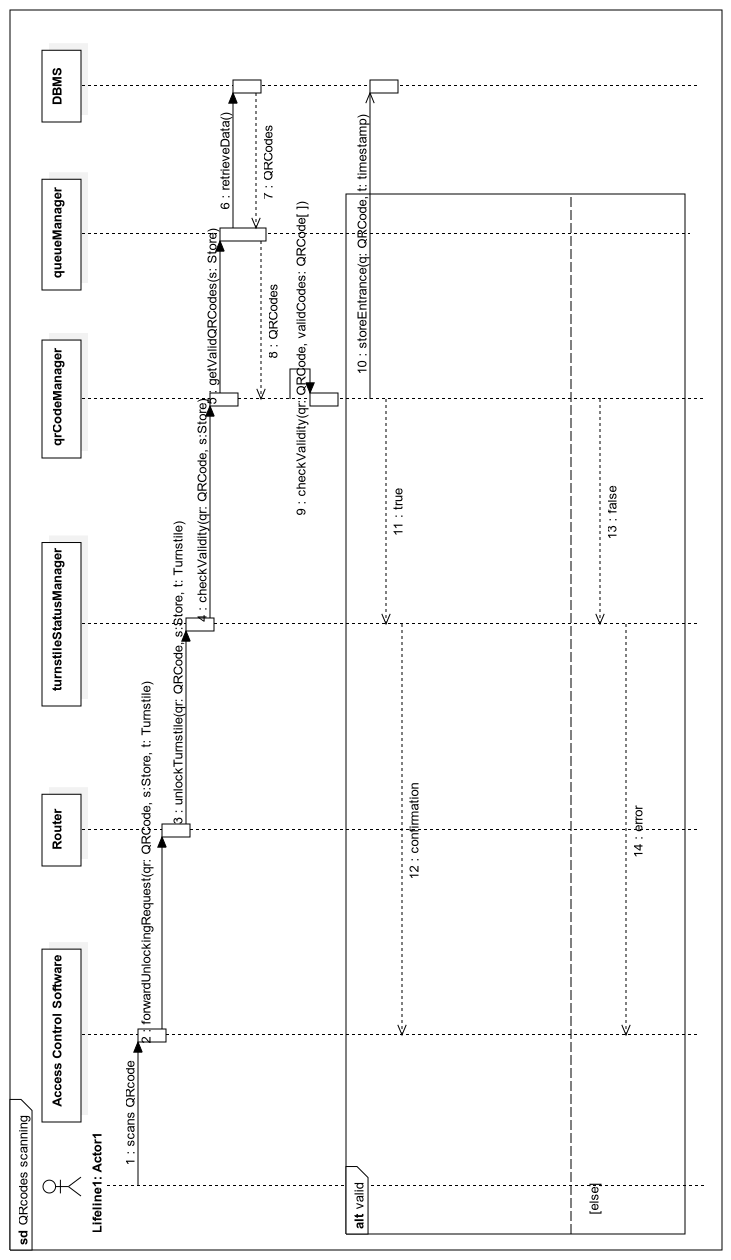
\includegraphics[width=\linewidth]{QrRT.png}
  
\end{figure}

\noindent The sequence diagram above describes which components’ interactions take place when a QR code is scanned by a turnstile. Whenever a store’s customer makes his/her QR code scanned, the turnstile’s Access Control Software forward a request to unlock the the turnstile (together with the scanned QR code informations) to the Router, which eventually forwards it to the TurnstileStatusManager. This last component handles the request by asking to the QRCodeManager, which communicates with the DBMS, to check the validity of the scanned QR code (not expired or false). If the check is successful, the TurnstileStatusManager is notified and a confirmation is sent to the Access Control Software, which eventually lets the turnstile unlock. Otherwise (unsuccessful check) the Access Control Software receives an error message and the turnstile will not be unlocked.
\subsection{Component Interfaces}
The following diagram shows the main components' interfaces, the interactions among them and the methods that can be invoked on them.
\begin{figure}[H]
  \includegraphics[width=\linewidth]{interfacesDiagram.png}
  
\end{figure}

\subsection{Selected architectural styles and patterns}

\noindent\textbf{Three Tier Client-Server}\\

\noindent As stated in the previous sections of this chapter, the chosen architecture for the system is the three tier one. It is a specific type of client-server system that provides many advantages in terms of development flexibility, scalability and security. Programmers indeed, can develop each tier independently and simultaneously, without affecting the other layers. Each tier can be scaled independently, when needed, and finally, the application tier makes the presentation and the data tiers communicate indirectly, making the overall treatment of data much safer. The presentation tier consists on the user interface, through which all the informations related to users’ lines and reservations are displayed. The CLup’s architecture, however, slightly deviates from the traditional three-tier architecture because of the piece of software deployed on the presentation tier itself, that handles the communication with the turnstile’s firmware.\\

\textbf{Model-View-Controller (MVC)}\\

\noindent In order to increase the system’s reusability and maintainability, the Model-View-Controller pattern has been selected. This software design pattern enables parallel development and makes the application’s development much faster. MVC is suitable for web and mobile applications, in particular in the context of an object-oriented programming style. The application is divided into three main logical components: the model, the view, and the controller, with the ultimate goal to separate the internal representations of informations from the way they are presented to the user.


\subsection{Algorithms}

\section{User Interface Design}
The application's mockups were presented in the RASD, more precisely in the user interface section. For this reason, the following UX diagrams are meant to provide a more detailed overview on the flow of UI screens that the users (both stores' customers and stores' managers) will follow to navigate inside the application (both mobile application or Web application).
\begin{figure}[H]
  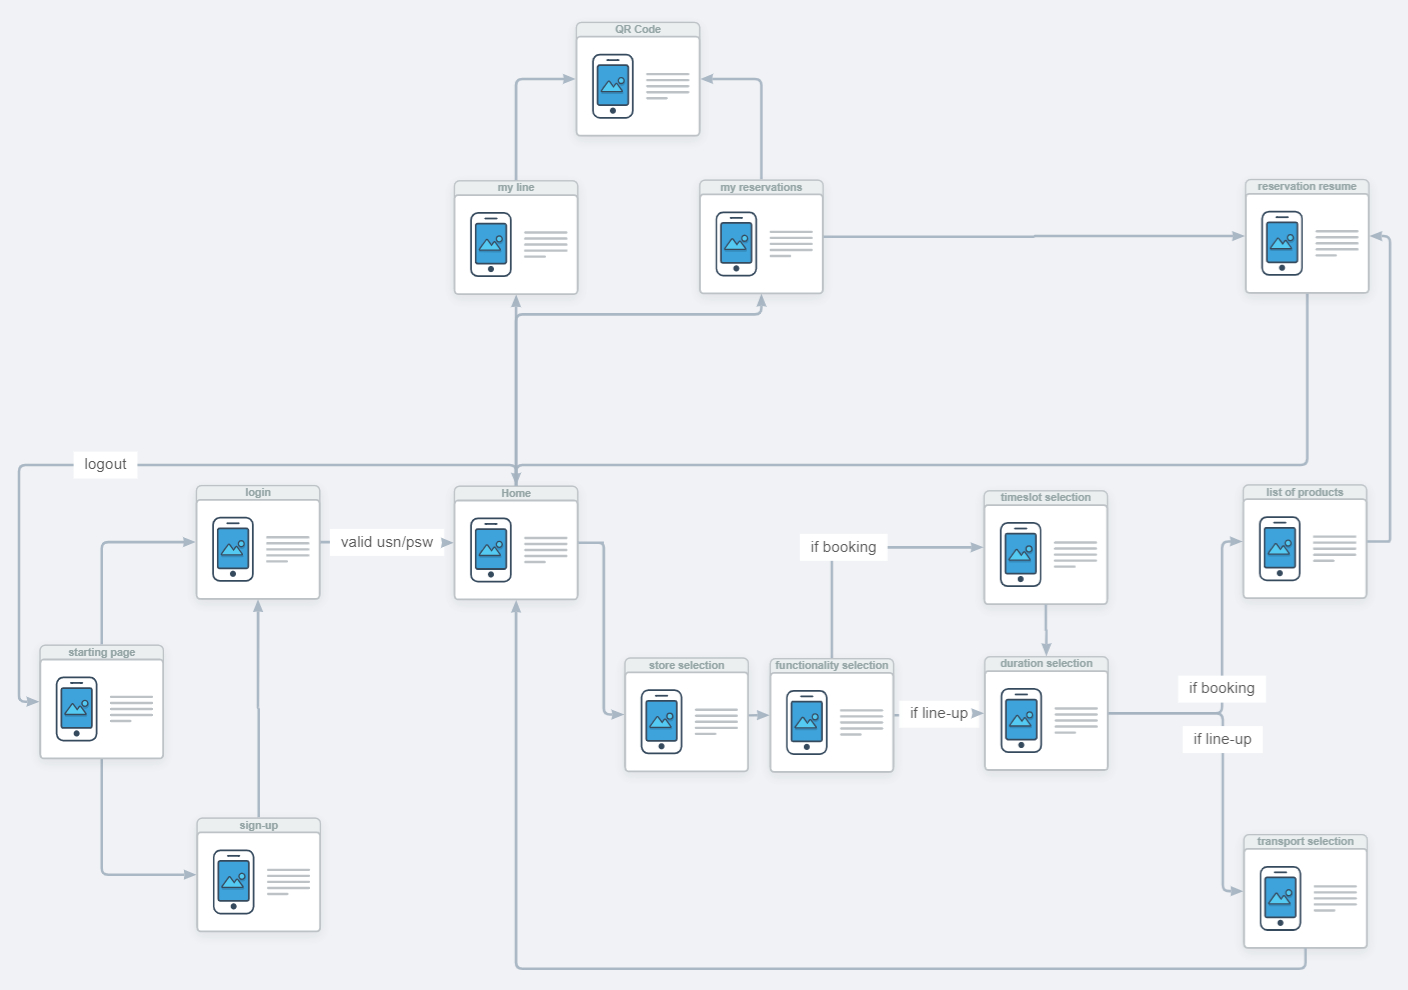
\includegraphics[width=\linewidth]{appUX.jpg}
  
\end{figure}
\begin{figure}[H]
  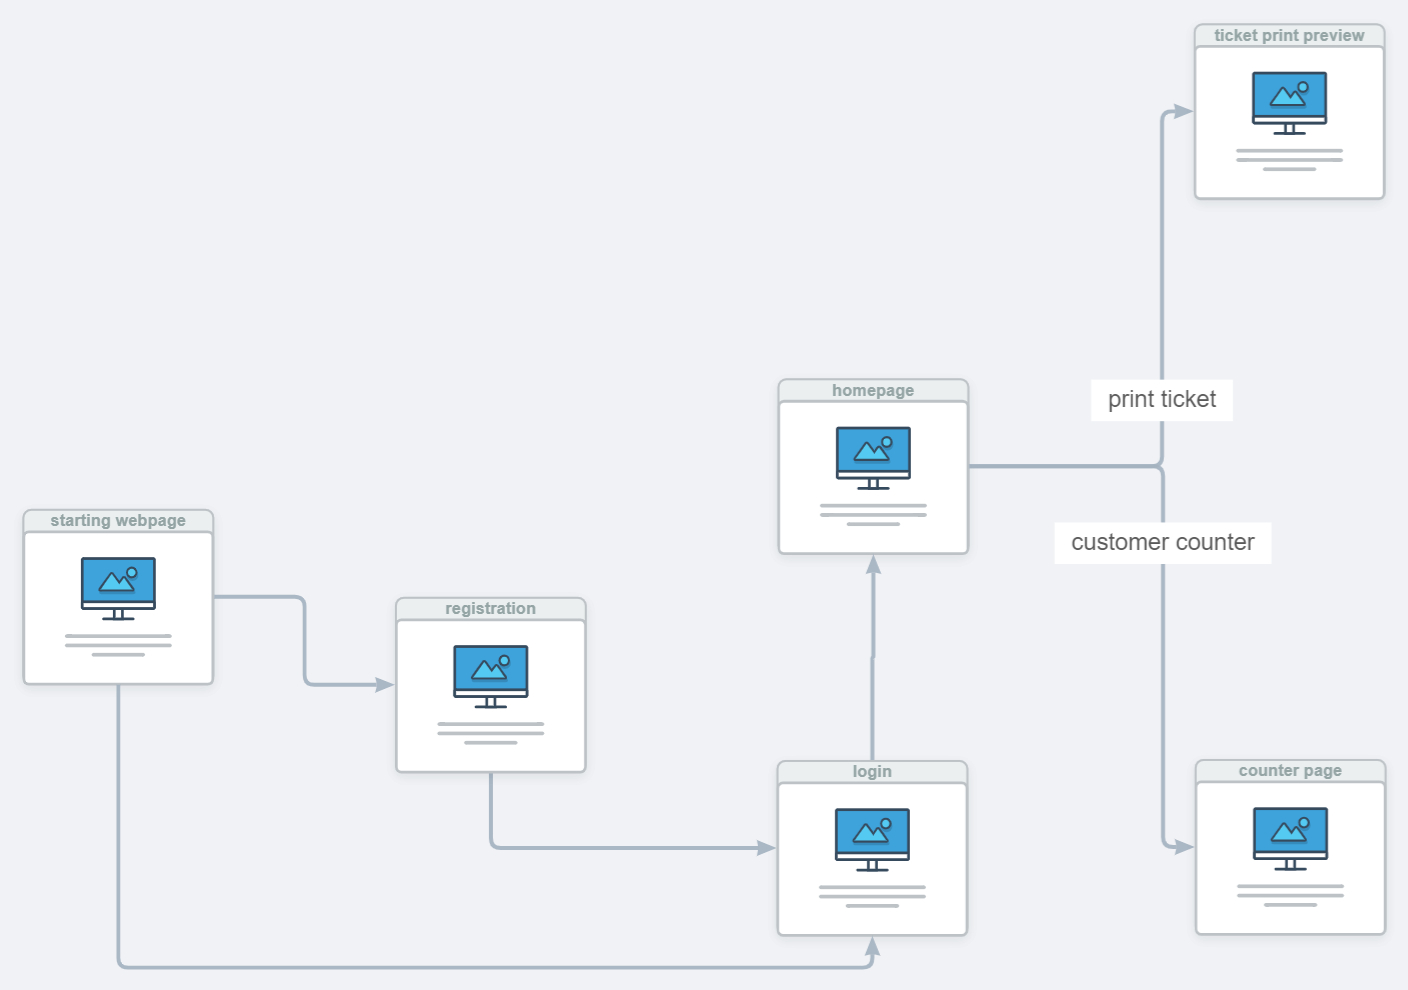
\includegraphics[width=\linewidth]{webUX.jpg}
  
\end{figure}

\section{Requirements Traceability}

\section{Implementation, Integration and Test Plan}
\subsubsection{Implementation}
The order in which the identified components will be implemented takes into account the fact that, in order for some of the components to work properly, some “core” components need to be implemented first. These dependancies among components mean that the best implementation, but also integration and testing approach to follow, is the bottom-up one. 
The application server’s components have higher priority, because the rest of the components rely on them.\\
\smallskip\\
CLup’s components can be grouped in the following way:\\
\smallskip\\
1. QueueManager and QrCodeManager\\
2. BookingManager and TurnstileStatusManager \\
3. TimeToArriveManager and MapsServiceMediator\\
4. TicketGenerationManager\\
5. LoginManager, SignUpManager, StoreRegistrationManager\\
6. Clients, Router and Access Control Software\\
\smallskip\\
The specified order corresponds to the order to follow for the implementation, integration and testing plans.\\
\smallskip\\
The \textbf{QueueManager} and the \textbf{QrCodeManager} have been chosen first because of their complexity and importance with respect to the other components. The QueueManager indeed, controls all the logic behind the virtual lines’ management, which is somehow affected by all the other CLup’s functionalities. The QR codes creation, managed by the QrCodeManager, is crucial for a proper functioning of virtual lines and reservations. For this reason, the QrCodeManager has to be implemented together with the QueueManager.\\
\smallskip\\
The same goes for the \textbf{BookingManager} and the \textbf{TurnstileStatusManager}. The former manages all the logic behind the booking process, while the latter needs to communicate with the QrCodeManager in order to handle the turnstiles’ status.\\
\smallskip\\
Once the components that enable a proper development of the core CLup’s functionalities have been implemented, components with lower priority are considered. In particular, the \textbf{TimeToArriveManager} in needed to manage all the informations related to the users’ location (distance and time to reach the stores). This component will be implemented but also integrated together with the \textbf{MapsServiceMediator}, which is the link between the whole system and the Google Maps Service.\\
\smallskip\\
In order to handle all the situations in which users that do not have access to the required technology interact with the system, the \textbf{TicketGenerationManager} is needed. This component as well communicates with the QueueManager.\\
\smallskip\\
The \textbf{LoginManager}, the \textbf{SignUpManager} and the \textbf{StoreRegistrationManager} are left at the end because, even if the functions provided by them are crucial for the entire system, the probability that something goes wrong while implementing them, is much lower with respect to the other components. Also, it is easier to estimate the time needed to complete them.\\
\smallskip\\
All the components that handles the communication between users and CLup’s services (\textbf{Clients}) and that redirects request to different parts of the system (\textbf{Router}) are finally implemented. The \textbf{Access Control Software} as well has been left at the end because implementing it in order to be compatible with just some specific turnstiles’  firmwares (the most common ones) will be reasonably straightforward. However, this particular component will be subject to continuous updating to make it compatible with new turnstiles’ types.\\
\smallskip\\
The Google Maps Service has not been mentioned because it represents an external system, that will be taken into account in the integration plan.
\section{Effort Spent}

\section{Reference Documents}

\end{document}